\chapter{Variantes de imitación}
\label{apx:il-curvas}

\lettrine{E}{ste} apéndice recoge las curvas de entrenamiento de las cuatro
variantes comparadas en la Iteración~II
(Capítulo~\ref{chap:iter2}) en la Tabla~\ref{tab:progresion-il} (página~\pageref{tab:progresion-il}),
todas bajo la misma configuración (igual partición e hiperparámetros, variando solo el
extractor). Se muestran juntas para ilustrar el sobreajuste que exhiben los modelos
dado el tamaño limitado del dataset de demostraciones y la similitud entre sus clases,
siendo la variante \gls{vit} el caso más pronunciado.

\begin{figure}[htbp]
  \vfill
  \centering
  \begin{minipage}{0.45\textwidth}
    \centering
    \textbf{\small Solo estado}\\[2mm]
    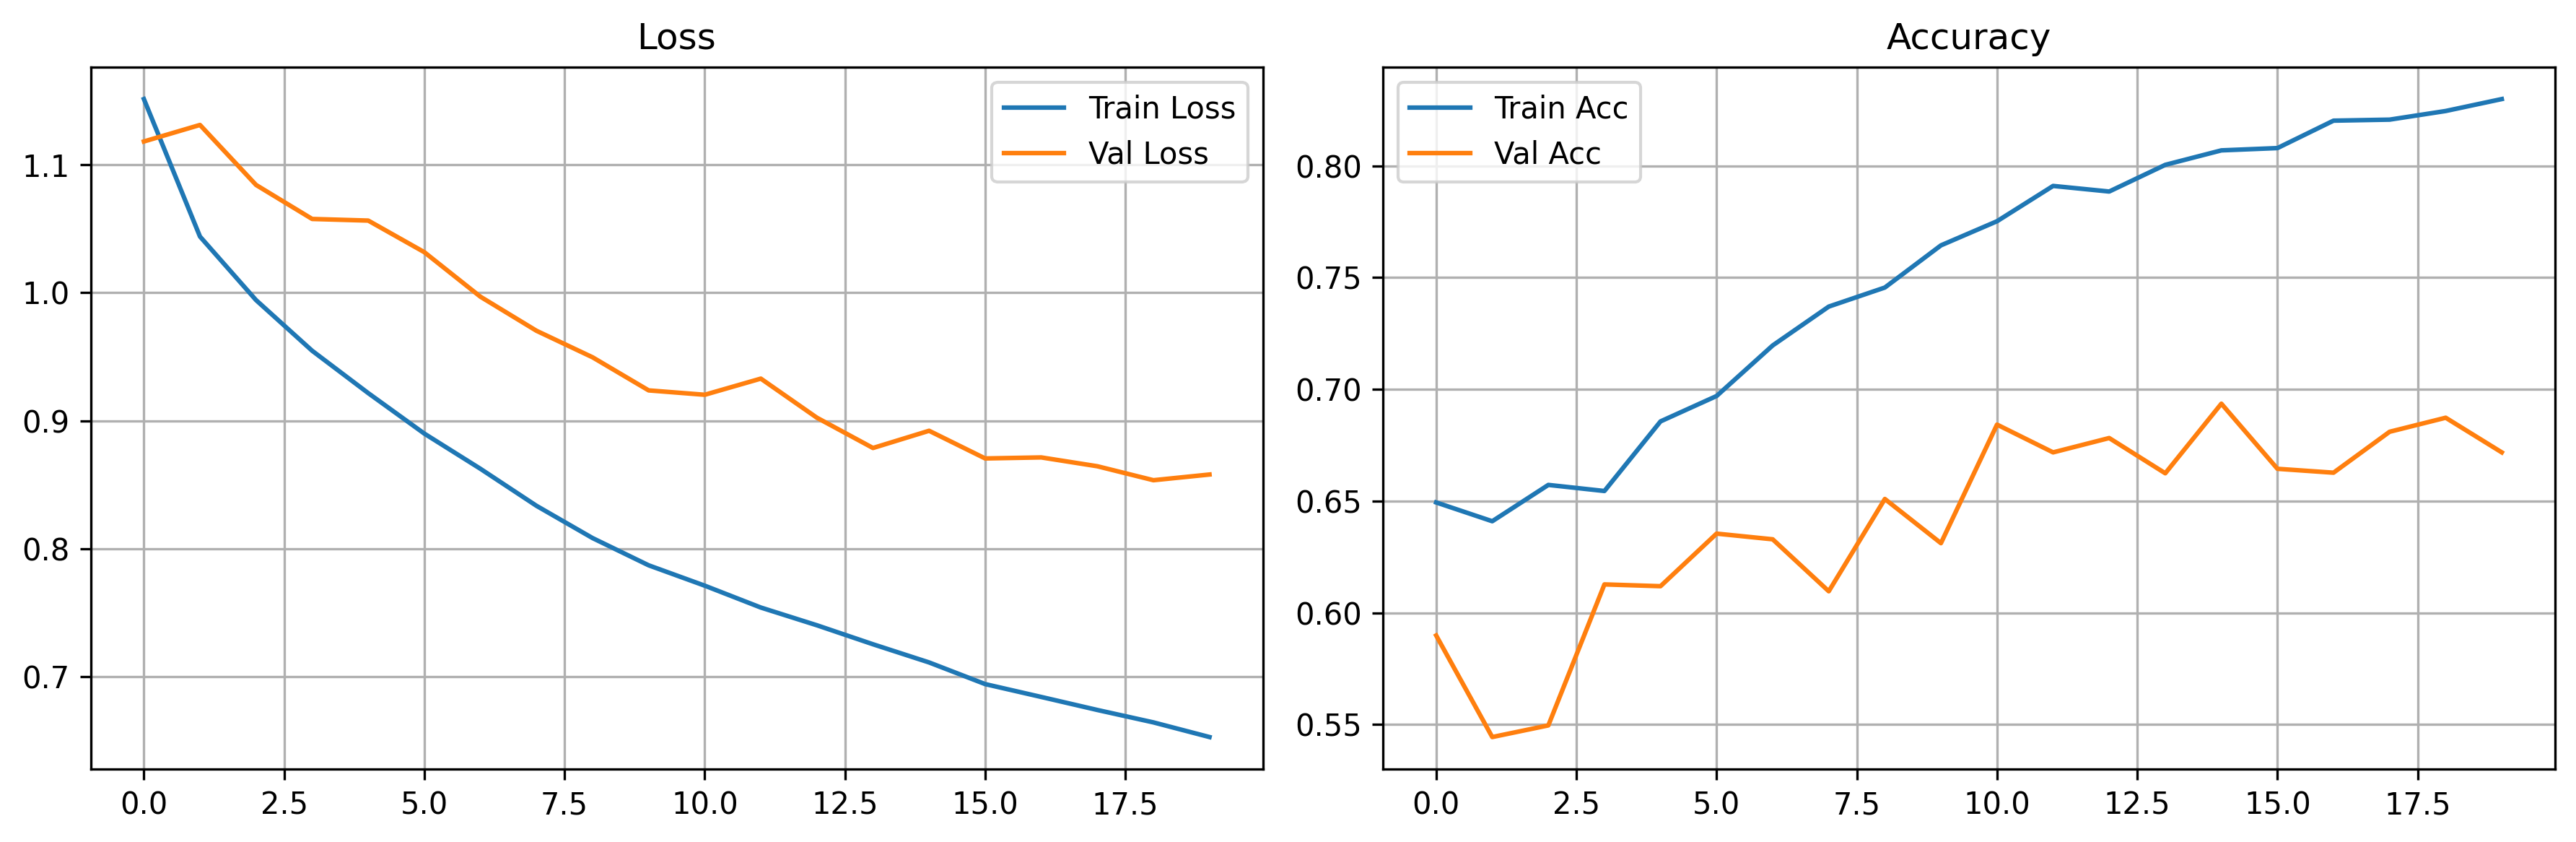
\includegraphics[width=\linewidth]{imaxes/anexos/il_curve_state.png}
  \end{minipage}\hfill
  \begin{minipage}{0.45\textwidth}
    \centering
    \textbf{\small Visual (\gls{gru})}\\[2mm]
    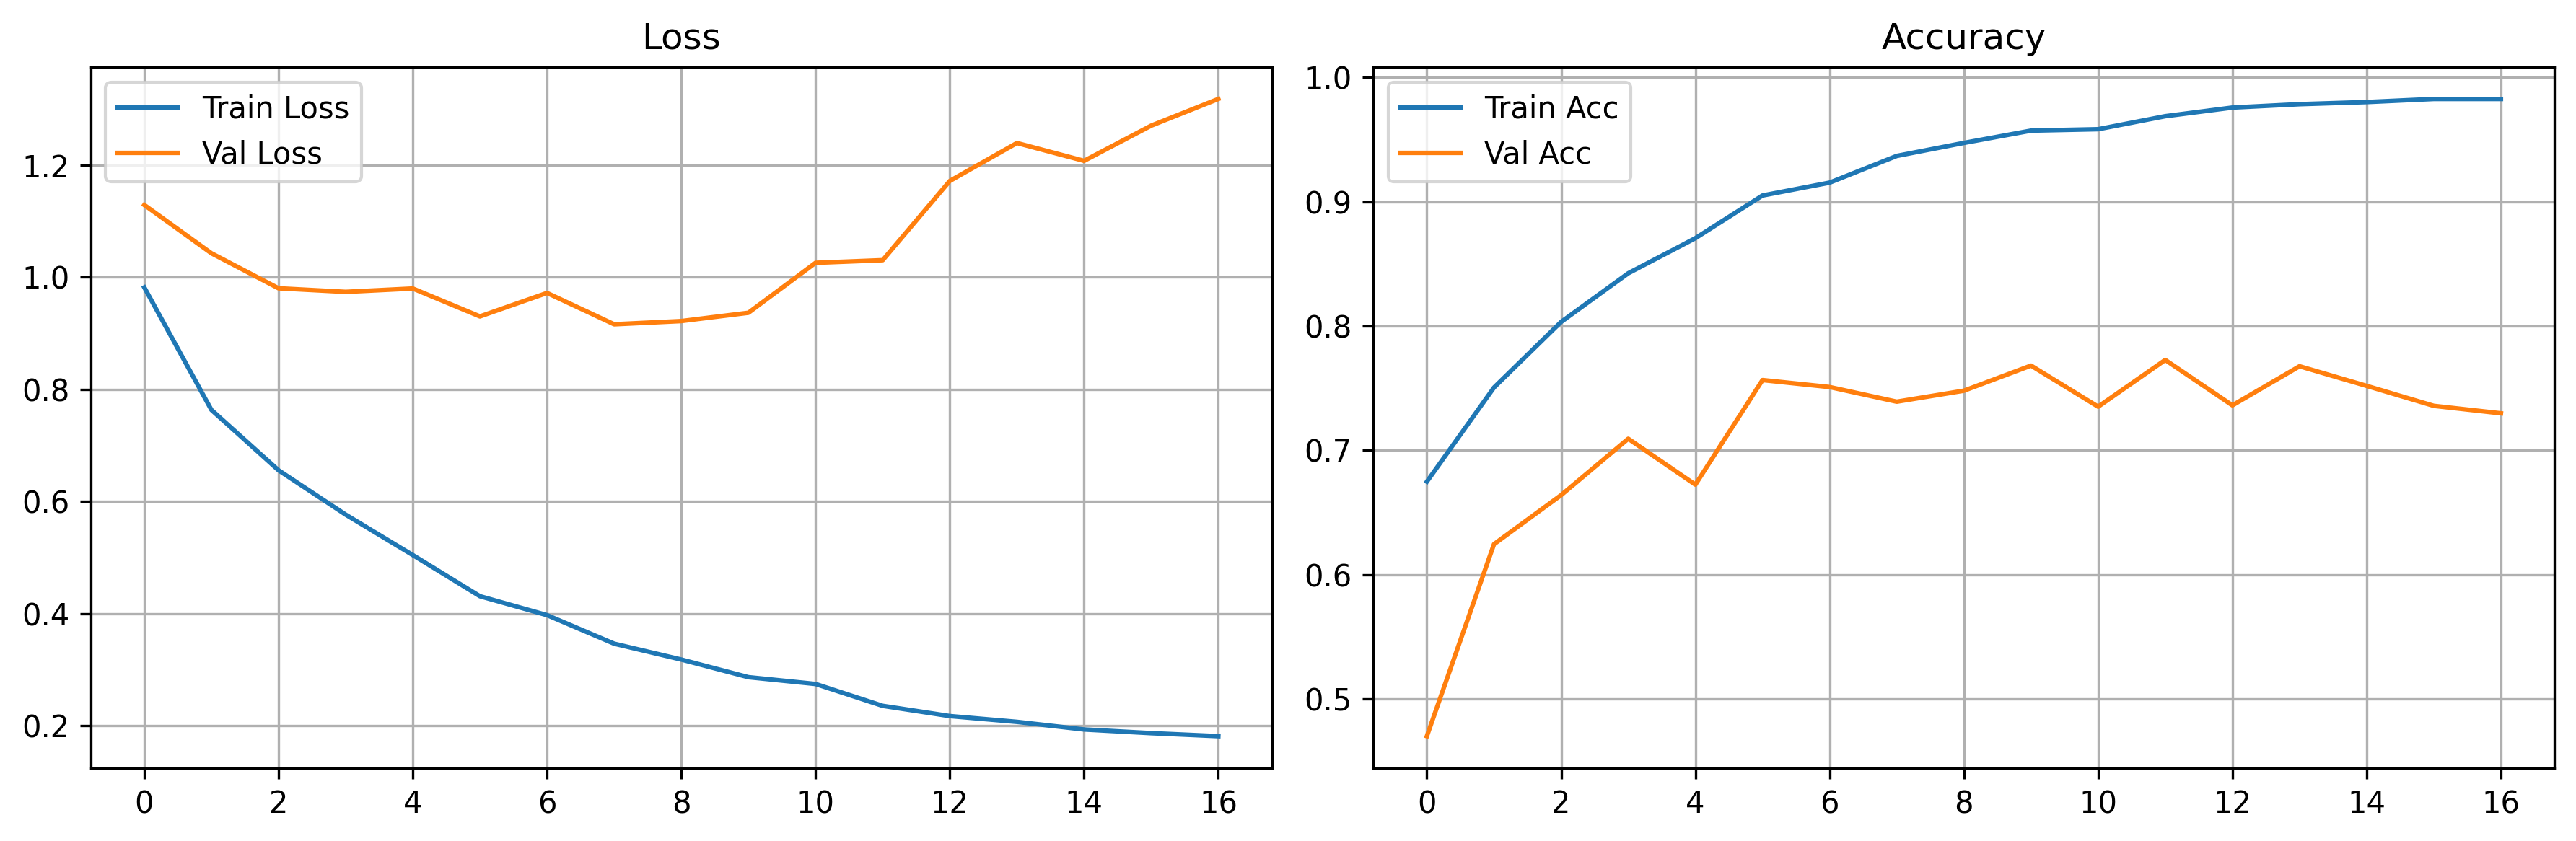
\includegraphics[width=\linewidth]{imaxes/anexos/il_curve_gru.png}
  \end{minipage}

  \vfill

  \begin{minipage}{0.45\textwidth}
    \centering
    \textbf{\small Visual (\gls{convlstm})}\\[2mm]
    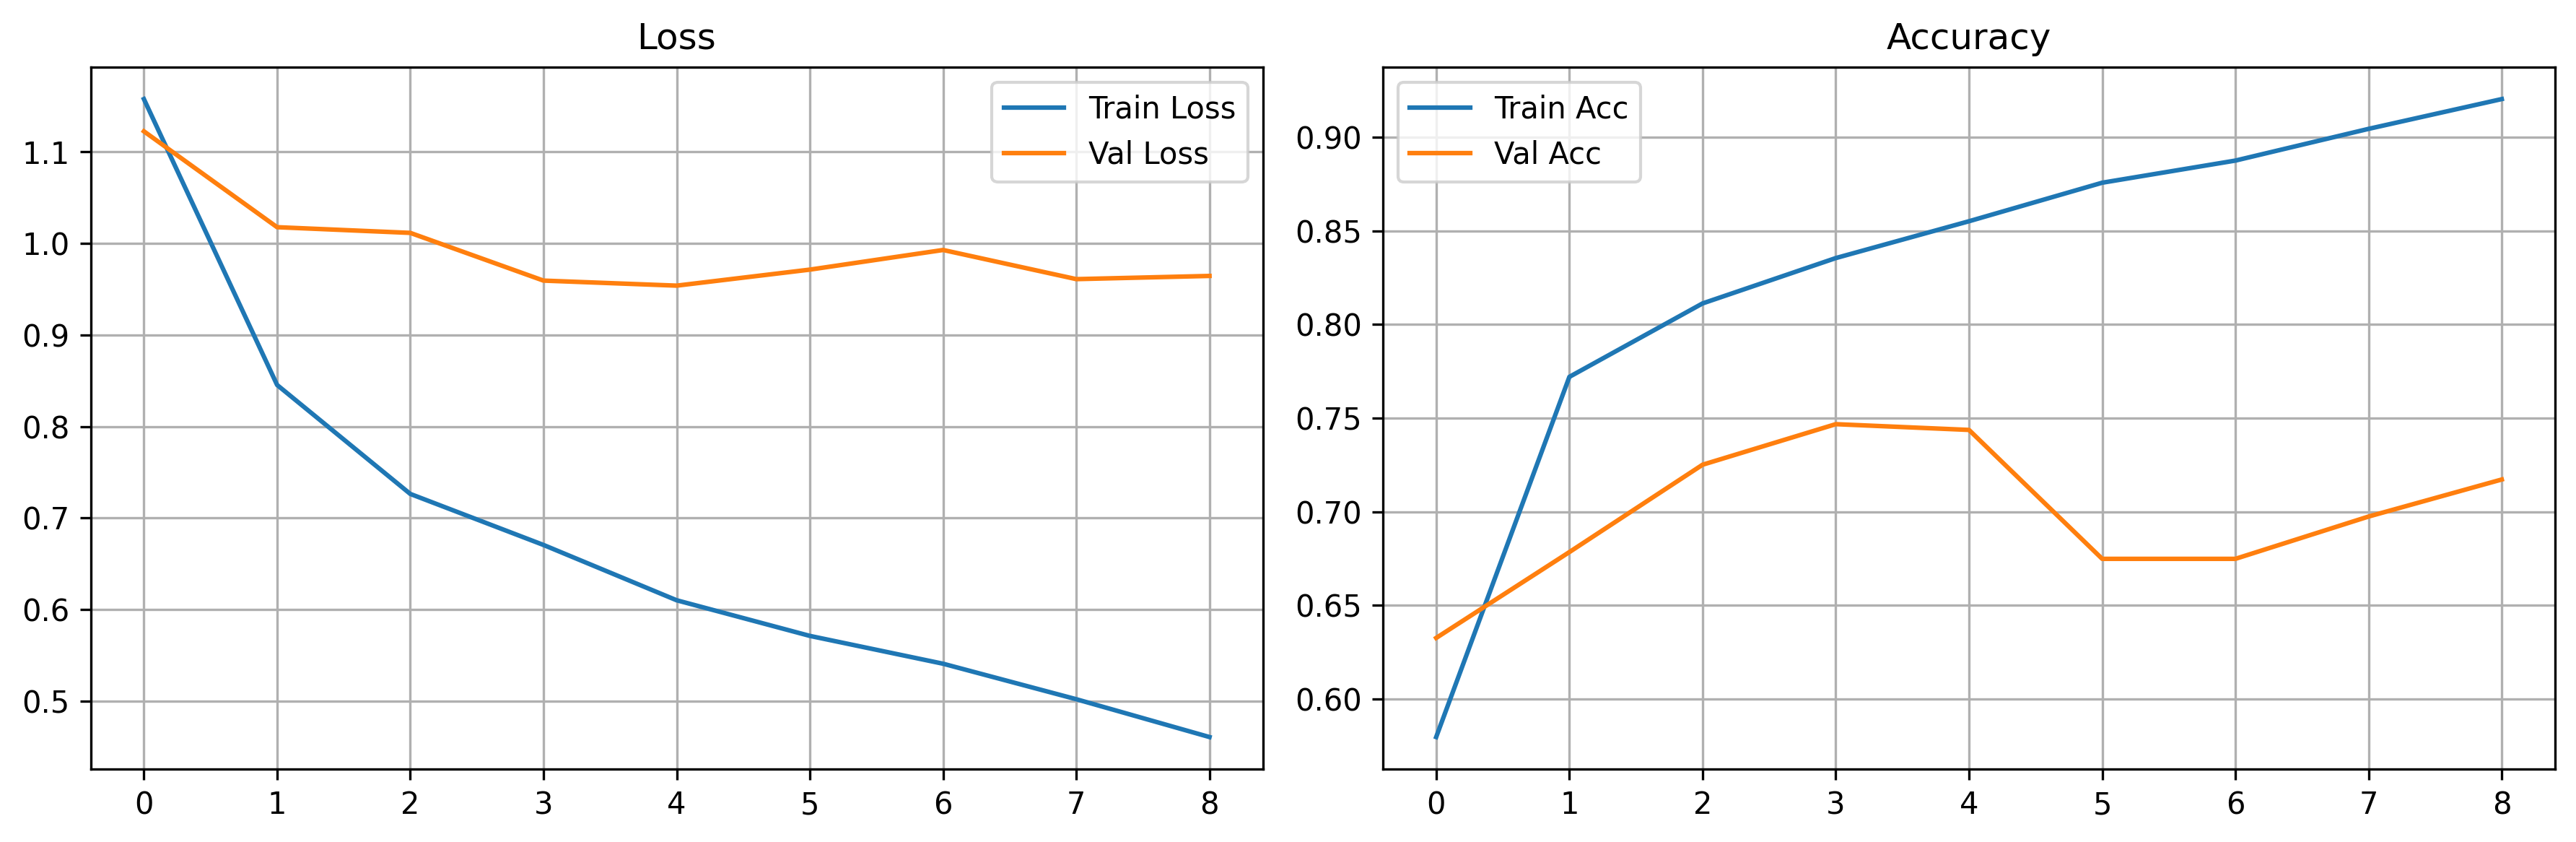
\includegraphics[width=\linewidth]{imaxes/anexos/il_curve_convlstm.png}
  \end{minipage}\hfill
  \begin{minipage}{0.45\textwidth}
    \centering
    \textbf{\small Visual (\gls{vit})}\\[2mm]
    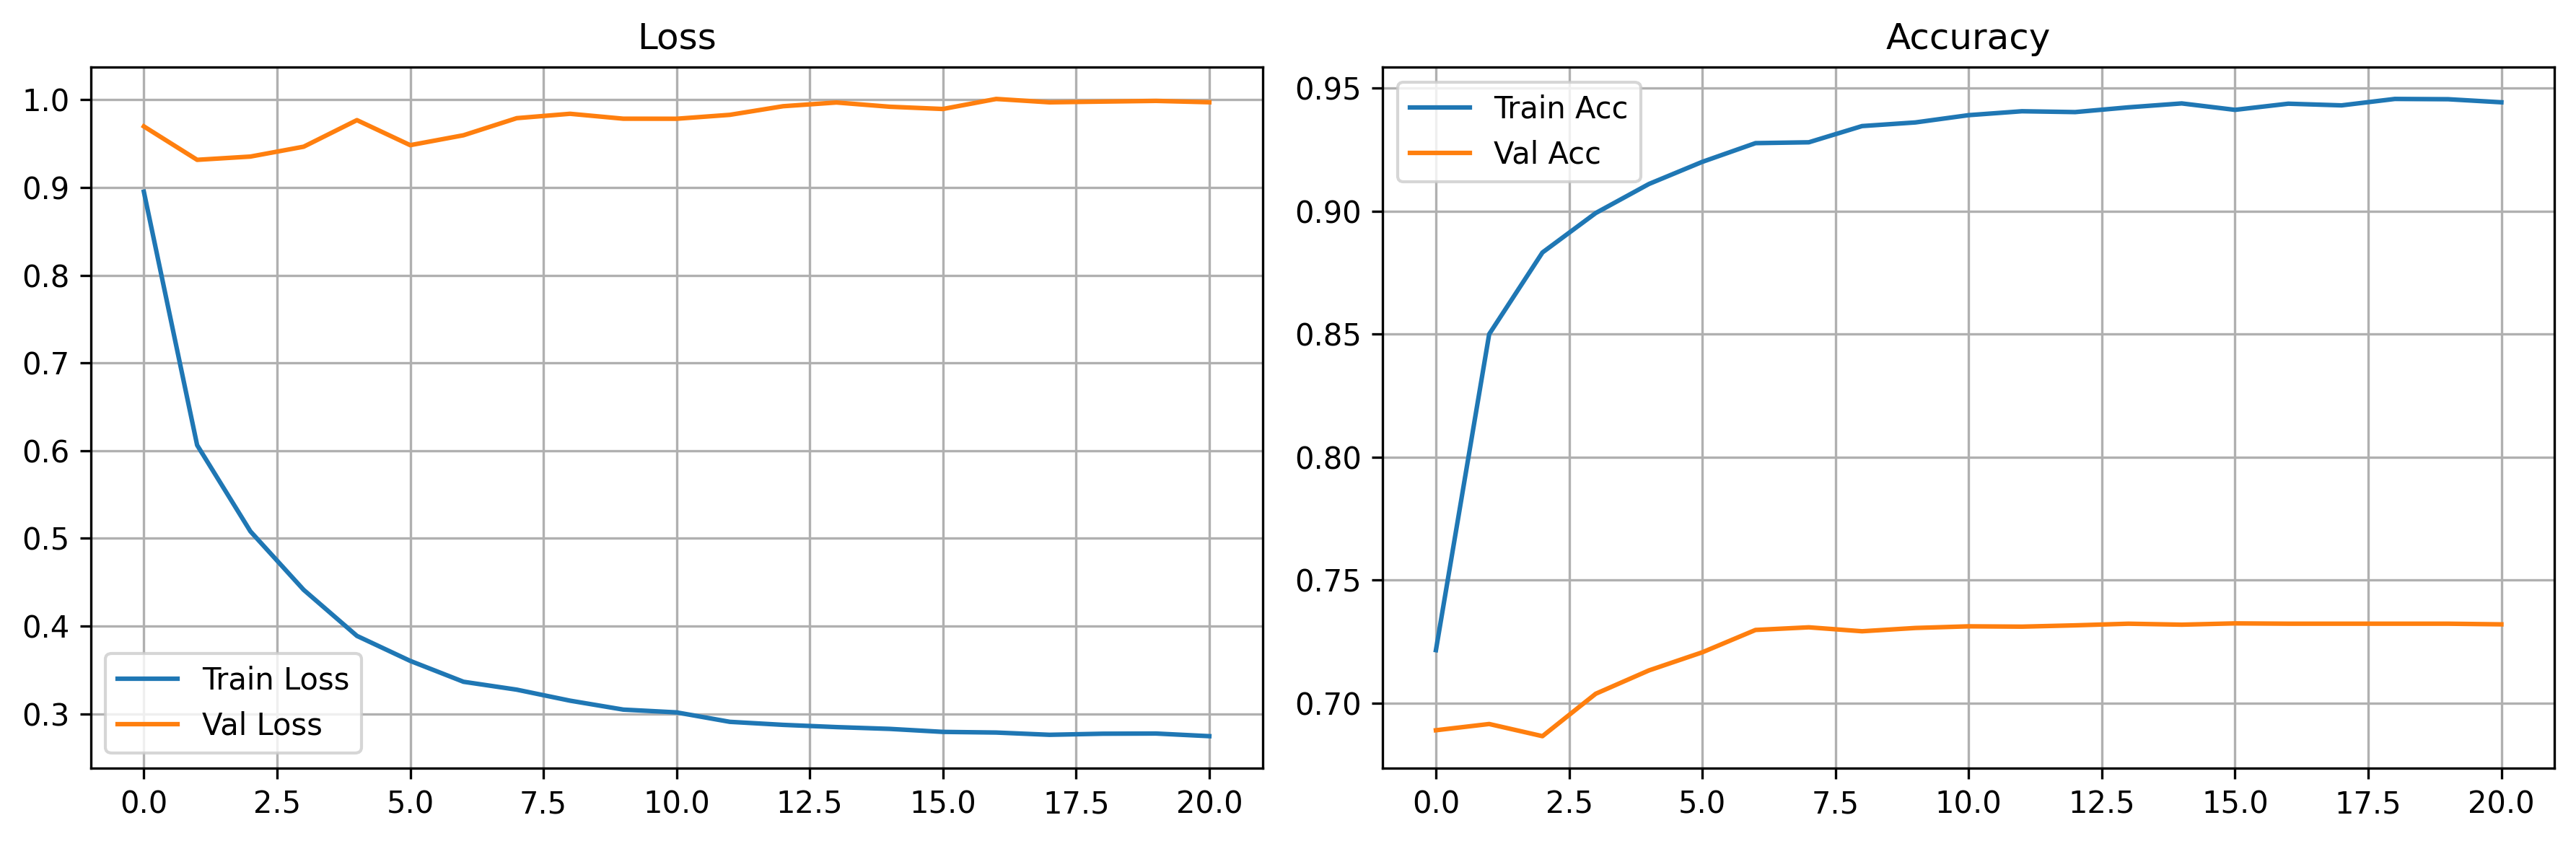
\includegraphics[width=\linewidth]{imaxes/anexos/il_curve_vit.png}
  \end{minipage}
  \vfill

  \caption[Curvas de entrenamiento de las variantes de imitación]{Curvas de
  entrenamiento (precisión y pérdida en entrenamiento y validación) de las cuatro
  variantes bajo configuración idéntica. El modelo de solo estado no alcanza
  una precisión de validación satisfactoria (cota inferior). Las variantes \gls{gru}
  y \gls{convlstm} generalizan de forma razonable, con una brecha
  entre entrenamiento y validación contenida. La variante \gls{vit} presenta el sobreajuste
  más pronunciado: su precisión de entrenamiento alcanza el ${\sim}$\num{95}\% mientras la
  de validación se estanca en torno al \num{72}--\num{73}\%, una brecha de más de \num{20}\%
  que evidencia que su mayor capacidad no se traduce en mejor generalización con un
  dataset de este tamaño.}
  \label{fig:apx-il-curvas}
\end{figure}
